\documentclass[aspectratio=169]{beamer}

% ── Packages ──────────────────────────────────────────────────────────────────
\usepackage{tikz}
\usetikzlibrary{arrows.meta,shapes.geometric,positioning,calc,fit,backgrounds}
\usepackage[T1]{fontenc}
\usepackage[utf8]{inputenc}
\usepackage{booktabs}
\usepackage{xcolor}
\usepackage{amsmath}

% ── Palette ───────────────────────────────────────────────────────────────────
\definecolor{accent}{RGB}{50,90,200}
\definecolor{accentmid}{RGB}{120,155,230}
\definecolor{accentlight}{RGB}{225,233,255}
\definecolor{ink}{RGB}{28,28,38}
\definecolor{mid}{RGB}{95,100,118}
\definecolor{rule}{RGB}{210,215,228}
\definecolor{nb}{RGB}{232,239,255}   % node blue fill
\definecolor{nbr}{RGB}{90,130,215}   % node blue border
\definecolor{ng}{RGB}{229,247,236}   % node green fill
\definecolor{ngr}{RGB}{50,160,90}    % node green border
\definecolor{no}{RGB}{255,244,228}   % node orange fill
\definecolor{nor}{RGB}{205,135,45}   % node orange border
\definecolor{arrc}{RGB}{70,105,190}

% ── Theme ─────────────────────────────────────────────────────────────────────
\usetheme{default}
\usefonttheme{professionalfonts}
\setbeamercolor{background canvas}{bg=white}
\setbeamercolor{normal text}{fg=ink}
\setbeamercolor{frametitle}{fg=ink,bg=white}
\setbeamercolor{itemize item}{fg=accent}
\setbeamercolor{itemize subitem}{fg=mid}
\setbeamercolor{block title}{fg=white,bg=accent}
\setbeamercolor{block body}{fg=ink,bg=accentlight}
\setbeamerfont{frametitle}{size=\large,series=\bfseries}
\setbeamerfont{framesubtitle}{size=\scriptsize,series=\normalfont}
\setbeamertemplate{navigation symbols}{}
\setbeamertemplate{itemize item}{\raisebox{0.15ex}{\small$\bullet$}}
\setbeamertemplate{itemize subitem}{--}
\setbeamersize{text margin left=18pt,text margin right=18pt}

% ── Frame title: left accent bar + thin rule ──────────────────────────────────
\setbeamertemplate{frametitle}{%
  \nointerlineskip
  \begin{beamercolorbox}[wd=\paperwidth,ht=1.4cm,dp=0pt]{frametitle}%
    \begin{tikzpicture}
      \fill[accent] (0,0) rectangle (4pt,1.4cm);
      \node[anchor=west,inner sep=0pt] at (12pt,0.7cm)
        {\begin{minipage}[c]{\dimexpr\paperwidth-28pt\relax}
          {\usebeamerfont{frametitle}\usebeamercolor[fg]{frametitle}\insertframetitle}%
          \ifx\insertframesubtitle\empty\else\\[1pt]%
            {\usebeamerfont{framesubtitle}\color{mid}\insertframesubtitle}\fi
        \end{minipage}};
    \end{tikzpicture}%
  \end{beamercolorbox}%
  {\color{rule}\hrule height 0.4pt}%
  \vskip4pt
}

% ── Footline ──────────────────────────────────────────────────────────────────
\setbeamertemplate{footline}{%
  \begin{beamercolorbox}[wd=\paperwidth,ht=14pt,dp=5pt]{normal text}%
    \hspace{18pt}{\color{mid}\tiny\textbf{JobMatch AI}}%
    \hfill{\color{mid}\tiny\insertframenumber\hspace{18pt}}%
  \end{beamercolorbox}%
}

% ── TikZ node styles ──────────────────────────────────────────────────────────
\tikzset{
  bn/.style={rectangle,rounded corners=5pt,draw=nbr,fill=nb,
    text width=#1,align=center,font=\small\bfseries,
    minimum height=0.9cm,inner sep=5pt},
  bn/.default=2.4cm,
  gn/.style={rectangle,rounded corners=5pt,draw=ngr,fill=ng,
    text width=#1,align=center,font=\small\bfseries,
    minimum height=0.9cm,inner sep=5pt},
  gn/.default=2.4cm,
  on/.style={rectangle,rounded corners=5pt,draw=nor,fill=no,
    text width=#1,align=center,font=\small\bfseries,
    minimum height=0.9cm,inner sep=5pt},
  on/.default=2.4cm,
  arr/.style={-{Stealth[length=5pt,width=4pt]},thick,color=arrc},
}

% ══════════════════════════════════════════════════════════════════════════════
\begin{document}
% ══════════════════════════════════════════════════════════════════════════════

% ── TITLE ─────────────────────────────────────────────────────────────────────
{
\setbeamertemplate{footline}{}
\setbeamertemplate{frametitle}{}
\begin{frame}
  \vfill
  \begin{tikzpicture}[remember picture,overlay]
    \fill[accent] (current page.south west) rectangle
      ([xshift=6pt]current page.north west);
  \end{tikzpicture}
  \hskip18pt
  \begin{minipage}{0.85\textwidth}
    \vspace{28pt}
    {\fontsize{34}{38}\selectfont\bfseries\color{ink} JobMatch AI}\\[8pt]
    {\large\color{mid} RAG-Powered Job Matching System}\\[30pt]
    {\small\color{mid} Applied Generative AI · FLAME University · April 2026}
    \vspace{28pt}
  \end{minipage}
  \vfill
\end{frame}
}

% ── OVERVIEW ──────────────────────────────────────────────────────────────────
\begin{frame}{Overview}
  \begin{columns}[t]
    \begin{column}{0.50\textwidth}
      \textbf{\color{accent}What we built}\\[6pt]
      An end-to-end AI job-matching platform. Upload a resume, describe your
      profile, and receive ranked job recommendations with personalised career
      advice, all grounded in real, retrieved job data.

      \vspace{10pt}
      \textbf{\color{accent}The problem}\\[6pt]
      Keyword search misses semantic fit.
      Pure LLMs hallucinate job details.
      \textbf{RAG} bridges both: retrieve real postings, then let the model
      reason over them.
    \end{column}
    \begin{column}{0.44\textwidth}
      \begin{block}{At a glance}
        \begin{itemize}\small\setlength{\itemsep}{3pt}
          \item 10{,}000+ Indian tech job listings
          \item Vector DB: Pinecone
          \item Gemma 3-27B response generation
          \item Resume parsing + cover letter
          \item Bookmarks \& application tracker
        \end{itemize}
      \end{block}
    \end{column}
  \end{columns}
\end{frame}

% ── DATASET ───────────────────────────────────────────────────────────────────
\begin{frame}{Dataset}
  \vspace{6pt}
  \begin{columns}[c]
    \begin{column}{0.48\textwidth}
      \begin{block}{Adzuna India Job Listings}
        \begin{itemize}\small\setlength{\itemsep}{4pt}
          \item \textbf{10,000} job postings ($\approx$7.1 MB CSV)
          \item Focus: Indian job market
          \item Fields: title, role, company, location,\\
                salary, experience, skills, sector,\\
                industry, description, benefits
        \end{itemize}
      \end{block}
    \end{column}
    \begin{column}{0.44\textwidth}
      \centering
      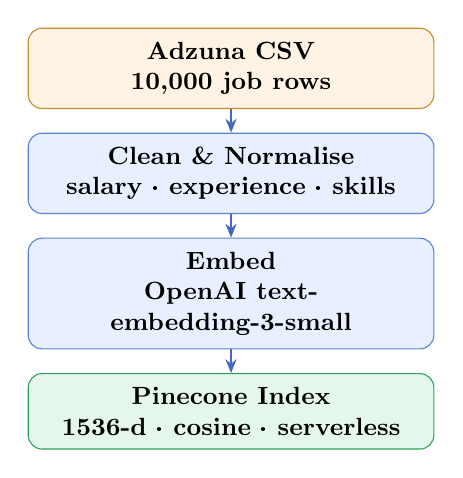
\begin{tikzpicture}[node distance=0.3cm]
        \node[on=4.8cm] (src) {\textbf{Adzuna CSV}\\{\small 10,000 job rows}};
        \node[bn=4.8cm,below=of src] (clean) {\textbf{Clean \& Normalise}\\{\small salary · experience · skills}};
        \node[bn=4.8cm,below=of clean] (emb) {\textbf{Embed}\\{\small OpenAI text-embedding-3-small}};
        \node[gn=4.8cm,below=of emb] (idx) {\textbf{Pinecone Index}\\{\small 1536-d · cosine · serverless}};
        \draw[arr] (src)--(clean);
        \draw[arr] (clean)--(emb);
        \draw[arr] (emb)--(idx);
      \end{tikzpicture}
    \end{column}
  \end{columns}
\end{frame}

% ── TECH STACK ────────────────────────────────────────────────────────────────
\begin{frame}{Tech Stack}
  \vspace{4pt}
  \centering
  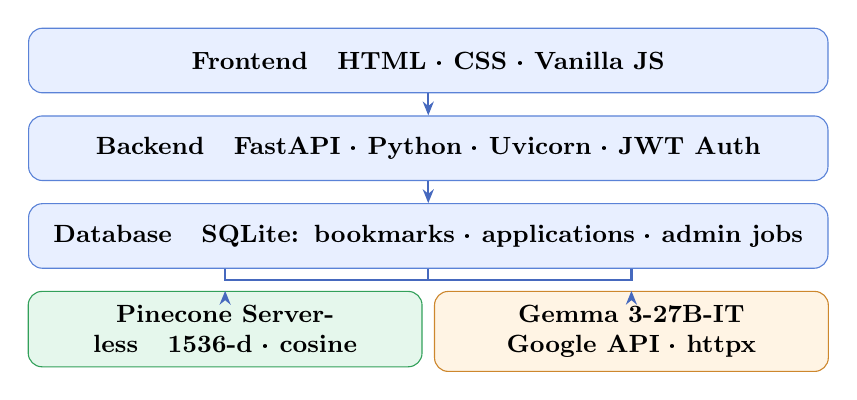
\begin{tikzpicture}[node distance=0.28cm]
    % Layer stack - centred
    \node[bn=9.8cm,minimum height=0.82cm] (fe)
      {\textbf{Frontend}\quad{\small HTML · CSS · Vanilla JS}};
    \node[bn=9.8cm,minimum height=0.82cm,below=of fe] (be)
      {\textbf{Backend}\quad{\small FastAPI · Python · Uvicorn · JWT Auth}};
    \node[bn=9.8cm,minimum height=0.82cm,below=of be] (db)
      {\textbf{Database}\quad{\small SQLite: bookmarks · applications · admin jobs}};

    % Two side-by-side bottom nodes
    \node[gn=4.65cm,minimum height=0.82cm,below=0.28cm of db,xshift=-2.58cm] (pc)
      {\textbf{Pinecone Serverless}\quad{\small 1536-d · cosine}};
    \node[on=4.65cm,minimum height=0.82cm,below=0.28cm of db,xshift=2.58cm] (llm)
      {\textbf{Gemma 3-27B-IT}\quad{\small Google API · httpx}};

    \draw[arr] (fe)--(be);
    \draw[arr] (be)--(db);
    \draw[arr] (db.south)--++(0,-0.14)-|([xshift=-2.58cm]db.south)--++(0,-0.14) (pc.north);
    \draw[arr] (db.south)--++(0,-0.14)-|([xshift=2.58cm]db.south)--++(0,-0.14) (llm.north);
  \end{tikzpicture}
\end{frame}

% ── PIPELINE ──────────────────────────────────────────────────────────────────
\begin{frame}{System Pipeline}
  \framesubtitle{Ingestion (top) · Query \& generation (bottom)}
  \vspace{6pt}
  \centering
  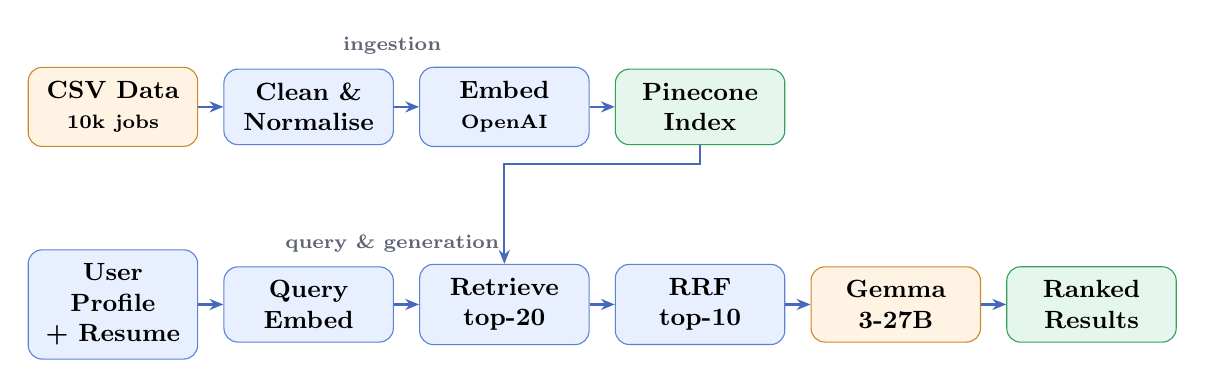
\begin{tikzpicture}[node distance=0.26cm and 0.32cm]

    % ── Ingestion row ──────────────────────────────────────────────────────────
    \node[on=1.8cm] (csv) {CSV Data\\{\scriptsize 10k jobs}};
    \node[bn=1.8cm,right=0.32cm of csv] (cl) {Clean \&\\Normalise};
    \node[bn=1.8cm,right=0.32cm of cl]  (em) {Embed\\{\scriptsize OpenAI}};
    \node[gn=1.8cm,right=0.32cm of em]  (pi) {Pinecone\\Index};

    \draw[arr] (csv)--(cl);
    \draw[arr] (cl)--(em);
    \draw[arr] (em)--(pi);

    \node[font=\scriptsize\bfseries\color{mid},above=0.06cm of cl,xshift=1.06cm]
      {\textsc{ingestion}};

    % ── Query row ─────────────────────────────────────────────────────────────
    \node[bn=1.8cm,below=1.3cm of csv]  (usr) {User Profile\\+ Resume};
    \node[bn=1.8cm,right=0.32cm of usr] (qe)  {Query\\Embed};
    \node[bn=1.8cm,right=0.32cm of qe]  (ret) {Retrieve\\top-20};
    \node[bn=1.8cm,right=0.32cm of ret] (rr)  {RRF\\top-10};
    \node[on=1.8cm,right=0.32cm of rr]  (gm)  {Gemma\\3-27B};
    \node[gn=1.8cm,right=0.32cm of gm]  (out) {Ranked\\Results};

    \draw[arr] (usr)--(qe);
    \draw[arr] (qe)--(ret);
    \draw[arr] (ret)--(rr);
    \draw[arr] (rr)--(gm);
    \draw[arr] (gm)--(out);

    \draw[arr] (pi.south)--++(0,-0.24)-|(ret.north);

    \node[font=\scriptsize\bfseries\color{mid},above=0.06cm of qe,xshift=1.06cm]
      {\textsc{query \& generation}};

  \end{tikzpicture}
\end{frame}


% ── RAG CONFIGURATION ─────────────────────────────────────────────────────────
\begin{frame}{RAG Configuration}
  \begin{columns}[t]
    \begin{column}{0.48\textwidth}
      \begin{block}{Retrieval}
        \begin{itemize}\small\setlength{\itemsep}{5pt}
          \item \textbf{Embedding}: OpenAI \texttt{text-embedding-3-small} (1536-d)
          \item \textbf{Search}: Pinecone cosine similarity, top-20
          \item \textbf{Reranking}: Reciprocal Rank Fusion (RRF) over 3 signals --- cosine rank, skill overlap rank, structural fit rank (location, seniority, work type, experience) $\to$ top-10
        \end{itemize}
      \end{block}
    \end{column}
    \begin{column}{0.46\textwidth}
      \begin{block}{Generation}
        \begin{itemize}\small\setlength{\itemsep}{5pt}
          \item \textbf{Model}: Gemma 3-27B-IT
          \item \textbf{Temperature}: 0.3
          \item \textbf{Max tokens}: 1{,}500
          \item \textbf{System prompt}: role definition, markdown schema, match scoring rubric (1--10)
        \end{itemize}
      \end{block}
    \end{column}
  \end{columns}
\end{frame}

% ── PROMPT INJECTION SAFETY ────────────────────────────────────────────────────
\begin{frame}{Safety \& Input Validation}
  \begin{columns}[t]
    \begin{column}{0.48\textwidth}
      \begin{block}{Resume Validation}
        \begin{itemize}\small\setlength{\itemsep}{5pt}
          \item PDF upload capped at \textbf{5 MB}
          \item Quality scored on email, headings, skills, dates; threshold score $\geq8$ and $\geq200$ chars
          \item Rejected before any LLM call is made
        \end{itemize}
      \end{block}
    \end{column}
    \begin{column}{0.46\textwidth}
      \begin{block}{Prompt Injection Defences}
        \begin{itemize}\small\setlength{\itemsep}{5pt}
          \item Control characters and null bytes stripped
          \item 10 injection phrases removed (``ignore all instructions'', ``jailbreak'', ``DAN'', etc.)
          \item XML role tags (\texttt{<system>}, \texttt{<user>}) stripped
          \item Field length caps on all user-controlled text
        \end{itemize}
      \end{block}
    \end{column}
  \end{columns}
\end{frame}

% ── EVALUATION ─────────────────────────────────────────────────────────────────
\begin{frame}{Evaluation}
  \framesubtitle{19 runs · 10 user profiles · no human relevance labels; proxy signals used throughout}
  \vspace{4pt}
  \begin{columns}[t]
    \begin{column}{0.48\textwidth}
      \textbf{\color{accent}Retrieval} \textnormal{\small(relevance proxy: cosine $\geq$ median)}\\[6pt]
      \begin{itemize}\small\setlength{\itemsep}{6pt}
        \item \textbf{Precision@K}: fraction of top-K above median cosine threshold\\
          {\footnotesize P@3\,=\,1.0 \enspace P@5\,=\,1.0 \enspace P@10\,=\,0.93}
        \item \textbf{NDCG@K}: position-weighted ranking quality; relevance grades = Gemma match scores\\
          {\footnotesize NDCG@10\,=\,0.69 (with \& without reranking)}
      \end{itemize}
    \end{column}
    \begin{column}{0.46\textwidth}
      \textbf{\color{accent}Generation quality}\\[6pt]
      \begin{itemize}\small\setlength{\itemsep}{6pt}
        \item \textbf{Faithfulness\,=\,1.0}: every recommended job was present in the retrieved set; no hallucinated listings across all 19 runs
        \item \textbf{Format consistency\,=\,0.75}: 6 of 8 output rules pass at 100\%; 2 fail due to Gemma heading style variability
        \item \textbf{Diversity}: company 0.69 \enspace location 0.40
        \item \textbf{Latency}: retrieval $\sim$2.1\,s \enspace generation $\sim$30\,s
      \end{itemize}
    \end{column}
  \end{columns}
\end{frame}

% ── LIMITATIONS ───────────────────────────────────────────────────────────────
\begin{frame}{Limitations}
  \vfill
  \centering
  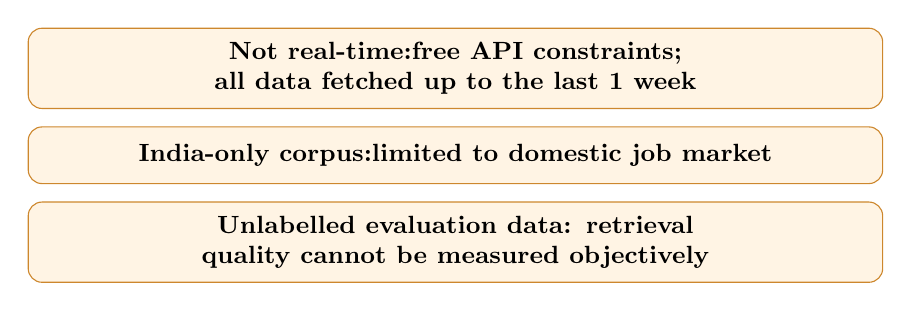
\begin{tikzpicture}[node distance=0.22cm]
    \node[on=10.5cm,minimum height=0.72cm] (l1)
      {\textbf{Not real-time}:free API constraints; all data fetched up to the last 1 week};
    \node[on=10.5cm,minimum height=0.72cm,below=of l1] (l2)
      {\textbf{India-only corpus}:limited to domestic job market};
    \node[on=10.5cm,minimum height=0.72cm,below=of l2] (l3)
      {\textbf{Unlabelled evaluation data}: retrieval quality cannot be measured objectively};
  \end{tikzpicture}
  \vfill
\end{frame}

% ── CLOSING ───────────────────────────────────────────────────────────────────
{
\setbeamertemplate{footline}{}
\setbeamertemplate{frametitle}{}
\begin{frame}
  \vfill
  \begin{tikzpicture}[remember picture,overlay]
    \fill[accent] (current page.south west) rectangle
      ([xshift=6pt]current page.north west);
  \end{tikzpicture}
  \hskip18pt
  \begin{minipage}{0.85\textwidth}
    \vspace{60pt}
    {\fontsize{40}{44}\selectfont\bfseries\color{ink} Thank You}
    \vspace{60pt}
  \end{minipage}
  \vfill
\end{frame}
}

\end{document}
